\documentclass{beamer}
\usetheme{default}
\usepackage{microtype}
\usepackage{graphicx}
\title{The Role of Bartle’s Gamer Types in Gamified Higher Education}
\author{William Seymour}
\institute{University of Warwick}
\date{March 12th, 2015}
\beamertemplatenavigationsymbolsempty

\begin{document}
	\begin{frame}
		\titlepage
	\end{frame}
	\frame{
		\frametitle{Presentation Overview}
		\begin{enumerate}
			\item What is gamification?
			\item What are Bartle's gamer types?
			\item Research undertaken
			\item Conclusion and further work
			\item Project evaluation
		\end{enumerate}
	}
	
	\frame{
		\frametitle{Gamification}
		\begin{quotation}
			``The use of game design elements \\ in non-game contexts''\footnote{Definition from “From game design elements to gamefulness by Detarding et al. (2011)}
		\end{quotation}
		
		Or, put another way, transplanting the game mechanics that make games engaging into other media with the aim of driving engagement.
		\newline
		
		It is important here to make the distinction between \textit{games} and \textit{gamified activities}. Not interested in things like controller support or fancy 3D graphics that typify game experiences.
	}
	
	\frame{
		\frametitle{Gamification}
		Though it existed since 2002, the term really spiked in usage from \textasciitilde2010\footnote{Google Trends image: proportion of gamification searches relative to the peak}. Gamification has psychological roots in operant conditioning (cf. B. F. Skinner) and Self Determination Theory.
		
			\begin{figure}
				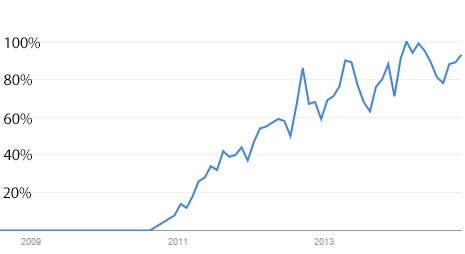
\includegraphics[width=0.5\linewidth]{../img/usage-graph.png}
			\end{figure}
			
			Usage of time over skill as a method of determining worth makes all players feel involved instead of just the top few.
	}
	
	\frame{
		\frametitle{Learning Analytics}
		The concept of using data analysis to inform the education process, giving a more personalised experience for students. Makes it possible to match students together by ability or learning style.
		\newline
		
		More popular than gamfication in HE, possibly due to the rise of big data.
		
		\begin{figure}
			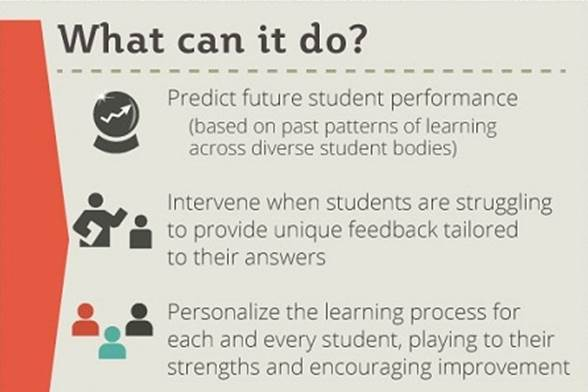
\includegraphics[width=0.6\linewidth]{../img/infographic.jpg}
			\footnote{Image part of an infographic by www.opencolleges.edu.au}
		\end{figure}
	}
	
	\frame{
		\frametitle{What does gamified higher education look like?}

		Uses a combination of gamification and learning analytics to enrich all aspects of campus life - from learning to sport and healthy eating.
		\newline
		
		We already have mechanisms for tracking visits to food outlets, so why not extend that and reward students for eating healthily? What data can we get from student cards and SSO?
		
		\begin{figure}
			
\includegraphics[width=0.5\linewidth]{../img/horizon.png}
		\end{figure}
		
		Would students be more inclined to study if they knew everyone else was putting in more effort?		
	}
	
	\frame{
	\frametitle{Bartle's Gamer Types}
	
	Proposed by Richard Bartle in his 1996 paper, the model categorises players into Socialisers, Killers, Achievers and Explorers. It acts as a way of psychologically profiling gamers based on their thoughts and actions in-game.
	
	\begin{center}
	\begin{tabular}{|c|c|c|}
		\hline - & Acting & Interacting \\ 
		\hline Players & Killers & Socialisers \\ 
		\hline World & Achievers & Explorers \\ 
		\hline 
	\end{tabular} 
	\end{center}
	
	Bartle refined this model in a later paper, but as only explicit and implicit variants of the above roles were added, along with adjustments for players changing over time, the project focuses on the simpler version.
	}
	
	\frame{
	\frametitle{Bartle's Gamer Types}	
		Bartle types can be used to reason about ecosystems of players in online multiplayer games. For example, the effect on the player base of increasing one type of user can be seen below.\footnote{Image from ``Hearts, clubs, diamonds, spades'' by Richard Bartle (1996).}
		\newline
		
		Despite being designed for MUDs (and by extension, MMOs), the Bartle types have found their way into a large amount of books and papers on gamification.
		
		\begin{figure}
			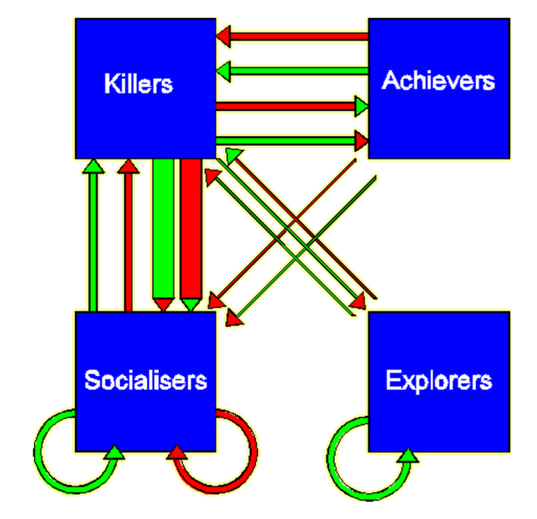
\includegraphics[width=0.5\linewidth]{../img/bartle.png}
		\end{figure}
	}
	
	\frame{
	\frametitle{Summary}	
	So, we've seen:
	\begin{itemize}
		\item What gamification is, and how it can be used in HE
		\item What Bartle's gamer types are, and what they are used for
	\end{itemize}

	\vspace{0.5cm}
	Which bring us nicely around to the original question:
	\begin{itemize}
		\item What place do Bartle's gamer types have in the future of gamified higher education?
	\end{itemize}
	}
	
	\frame{
	\frametitle{Research Undertaken}
	
	Begin by discussing ``Modeling the player, learner and personality'' by Konert et al\footnote{Johannes Konert, Stefan Gobel, and Ralf Steinmetz. Modeling the player, learner and personality: Independency of the models of bartle, kolb and neo-ffi (big5) and the implications for game based learning. 7th European Conference on Games Based Learning, 2013.}. The paper examines the link between the Bartle type and LSI/Big 5 scores of 12-14 year olds.
	\newline

	While a few correlations were found, there was nothing to evidence a larger pattern.
	
	\begin{quotation}
		``All in all, the results do not fulfill the expectations of the study. Predicting the playing style preferences based on the BFI-K profile of a gamer is only possible for the Socializer playing style''
	\end{quotation}	
	}
	
	\frame{
	\frametitle{Research Undertaken}	
		
		My project set out to follow up on this by:
		\begin{itemize}
			\item Taking a step back and examining correlations between gamer type and personality (non BFI)
			\item Explaining the correlation between the above, or lack thereof
		\end{itemize}
			
		\vspace{0.5cm}
		23 HE students, mainly from Warwick, completed profiling exercises for Bartle type and Keirsey Temperament.\footnote{Keirsey Temperament is a measure of personality, similar in scope to BFI} An online testing platform was constructed for the task, which was able to lessen the workload by automating some of the analysis.
	}
	
	\frame{
	\frametitle{Research Undertaken}	
	
		Raw results from participants were normalised over the interval (0,1). This equates to:
	
	\begin{center}
		$\frac{number\:of\:X\:reposes\:given}{total\:number\:of\:possible\:X\:responses}$
	\end{center}
	\vspace{0.5cm}
	
	These were then used to calculate the Pearson Product Moment Correlation Coefficient for each combination:
	
	\begin{center}
		$r=\frac{\sum_{i=1}^{n}(X_i-\bar{X})(Y_i-\bar{Y})}{\sqrt{\sum_{i=1}^{n}(X_i-\bar{X})^2}\sqrt{\sum_{i=1}^{n}(Y_i-\bar{Y})^2}}$
	\end{center}
	(With $\bar{X}$ and $\bar{Y}$ being the mean of $X$ and $Y$ respectively)
	\newline
	
	Alternatively put, this is the covariance of the
	two variables divided by the product of their standard deviations.
	}
	
	\frame{
	\frametitle{Research Results}
	
	\begin{figure}
		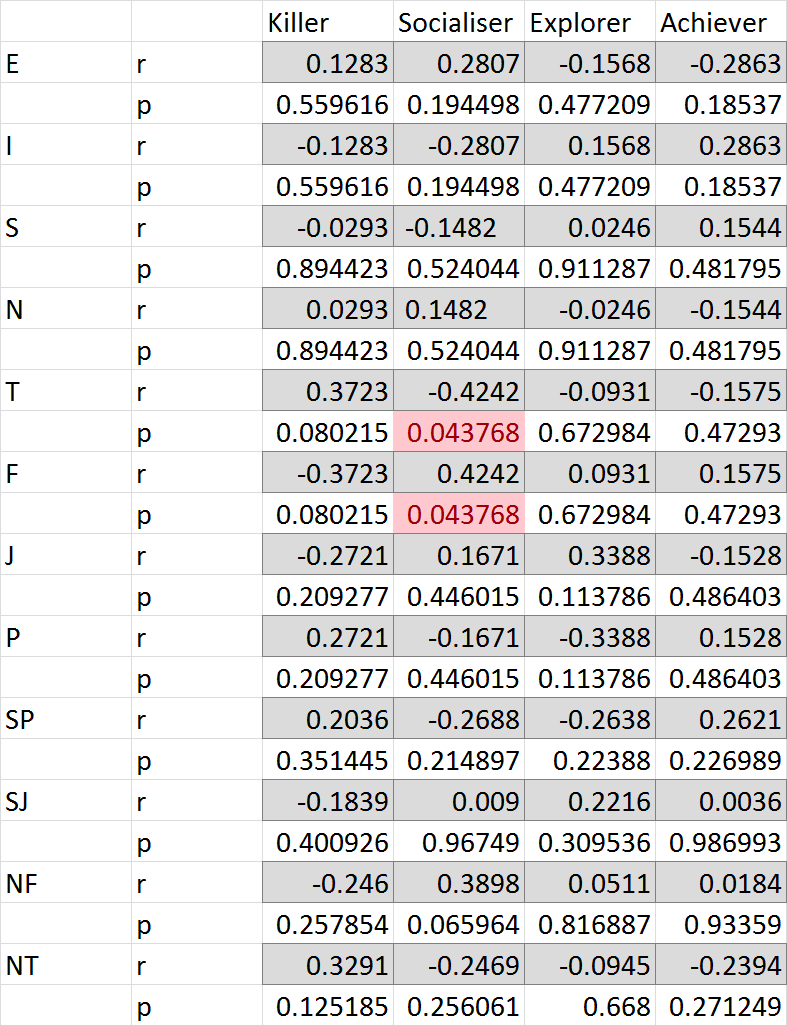
\includegraphics[width=0.55\textwidth]{../img/results.png}
	\end{figure}
	
	}
	
	\frame{
	\frametitle{Research Analysis}
		These findings echo those of Konert et al., including the rogue socialiser correlation.
		\newline
	
		This is understandable given the disposition of feeling types to be more personal when dealing with others and to respond more warmly in social situations. Furthermore, on	socialisers, Bartle writes that:
		
		\begin{quotation}
		``Finding out about people and getting to know them is far
		more worthy than treating them as fodder to be bossed around. The game world is just a
		setting; it's the characters that make it so compelling''	
		\end{quotation}
	}
	
	\frame{
	\frametitle{Research Analysis}
	
		In order to fully explain these findings we have to go back and re-examine the theory of games themselves. In 1961 Roger Callois described in his work ``Man, Play and Games'' a type of play he called \textit{mimicry}:
		\begin{quotation}
			``Play can consist not only of deploying actions or submitting to one's fate
			in an imaginary milieu, but of becoming an illusory character oneself, and of
			so behaving. One is then confronted with a diverse series of manifestations,
			the common element of which is that the subject makes believe or makes
			others believe that he is someone other than himself. \textbf{He forgets, disguises,
			or temporarily sheds his personality in order to gain another}''
		\end{quotation}
	}
	
	\frame{
	\frametitle{Conclusion}
	The question:
	\begin{itemize}
		\item What place do Bartle's gamer types have in the future of gamified higher education?
	\end{itemize}
	\vspace{0.5cm}
	
	From the background research and study results:
	\begin{itemize}
		\item Modelling metrics separately misses the point 
		\item Perhaps we should ask students who they \textit{would like to be}
		\item We should restrict use of Bartle types to the experiences for which they were designed
	\end{itemize}
		
	}
	
	\frame{
	\frametitle{Further Work}	
	
	\begin{itemize}
		\item The focus should be on how these metrics affect actual usage and engagement
		\item Direct efforts towards the relationship between learning style and task preference (Schaller et al.)
	\end{itemize}
		
	}
	
\end{document}